% This is samplepaper.tex, a sample chapter demonstrating the
% LLNCS macro package for Springer Computer Science proceedings;
% Version 2.20 of 2017/10/04
%
\documentclass[runningheads]{llncs}
%
\usepackage{graphicx}
% Used for displaying a sample figure. If possible, figure files should
% be included in EPS format.
%
% If you use the hyperref package, please uncomment the following line
% to display URLs in blue roman font according to Springer's eBook style:
% \renewcommand\UrlFont{\color{blue}\rmfamily}

\usepackage{subcaption}
\usepackage[T1]{fontenc}
\usepackage{nameref}

\renewcommand{\arraystretch}{1.2}
\setlength\tabcolsep{1.75pt}

\begin{document}
%
\title{Diabetes Patients Early Readmission Prediction}
%
%\titlerunning{Abbreviated paper title}
% If the paper title is too long for the running head, you can set
% an abbreviated paper title here
%
\author{Peter Mačinec \and
František Šefčík}
%
\authorrunning{P. Mačinec, F. Šefčík}
% First names are abbreviated in the running head.
% If there are more than two authors, 'et al.' is used.
%
\institute{Faculty of Informatics and Information Technologies,\\Slovak University of Technology, Bratislava}
%
\maketitle              % typeset the header of the contribution
%
\begin{abstract}
Nowadays, more and more patients suffer from still incurable diabetes disease. Every wrong chosen treatment for patients can harm their health and lead to early readmission that costs more money. Therefore, there is a demand for predicting the readmission of patients to increase quality of health care and also to reduce costs. However, standard methods for identifying the patients with risk of readmission perform poorly (e.g. LACE index). With growing number of patients with diabetes, there is a need for methods that can automatically and more accurate predict the readmission. In this paper, we provide method based on machine learning for predicting early readmission of patient. The results of data analysis and machine learning methods showed that there is a potential of using data-driven approach for this problem.

\keywords{diabetes \and early readmission prediction \and machine learning \and data analysis.}
\end{abstract}


\section{Motivation}

Diabetes is a wide spread chronic disease that is related to irregular blood glucose levels caused by problems with insulin. The number of people with diabetes has increased enormously in recent years and costs for health care with each hospital admission are rising simultaneously. The methods of diabetes treatment of patient have high impact on mortality and morbidity. Wrong treatment can endanger patient's health and may lead to early readmission.

A hospital readmission is when a patient who is discharged from the hospital, gets re-admitted again within certain period of time. By predicting readmission, more attention may be given to treatment of patients with high probability of readmission and so increase the quality of care during hospitalization. Because there is no cure for the diabetes yet\footnote{https://www.diabetes.org.uk/diabetes-the-basics/is-there-a-cure} and diabetic patients can be readmitted in the future, an \textit{early readmission prediction} can help mostly when it comes to selection of best treatment for the patient.

Data of patients clinical encounters are being collected naturally with healthcare systems, thus data-driven approach seem to be appropriate for this problem. Machine learning algorithms used for early readmission prediction provide ability to process the data of a lot of patients and may help to find hidden dependencies in the data to outperform basic methods (e.g. LACE index).

The task of \textit{early readmission prediction} can be represented as binary classification problem into two classes - patient was early readmitted or not. The term \textit{early readmission} is very relative. In our case, we define it as patient being readmitted in less than one month (30 days).


\section{Related works}

Task of predicting diabetic patients readmission is substantive from two points of view - health of patients and saving money because of readmission. Because data of patients are usually available from health records, much research has been done also in data mining area.

Majority of previous works in this area are based on traditional machine learning workflow, including data analysis, data preprocessing and modeling. However, the task defined can vary across researchers - some of them are trying to predict early patients readmission~\cite{Hammoudeh2018,Sharma2019,Mingle2017}, and then there is also work where authors are trying to predict short and long term readmissions~\cite{Bhuvan2016}. Different but interesting approach that was also the subject of research is to predict readission across age groups~\cite{Mingle2017}.

In the previous works, much effort has been spent on data preprocessing. Basic well-known steps of preprocessing like filtering useless columns, normalization, outliers removal and one-hot encoding were usually performed~\cite{Sharma2019,Mingle2017,Hammoudeh2018,Bhuvan2016}. Also heavy ensemble models have been tried instead of detailed preprocessing~\cite{Mingle2017}, but comparison of the achieved results with other works showed that the proper preprocessing always has its place in machine learning tasks.

Because the classes (patient was early readmitted or not) are naturally imbalanced, class balancing was usually performed. Oversampling was preferred over undersampling, and usually SMOTE (Synthetic Minority Over-sampling Technique) was used~\cite{Sharma2019,Hammoudeh2018}. From the analyzed works we can deduce that training machine learning algorithms after data oversampling leads to better results.

When it comes to modeling, many different approaches and methods were used. Mostly used were tree-based algorithms, like random forest~\cite{Sharma2019,Bhuvan2016}, decision tree~\cite{Sharma2019} or xgboost~\cite{Sharma2019}. Also, other algorithms were tried, e.g. logistic regression~\cite{Sharma2019}, Adaboost~\cite{Sharma2019,Bhuvan2016}, naive Bayes~\cite{Bhuvan2016}. Neural networks are not so popular in this area, but for example multi-layer perceptron~\cite{Bhuvan2016} or convolutional neural networks~\cite{Hammoudeh2018} were used. In general, tree-based models (and mostly random forest) alongside with convolutional neural networks achieved the best results - accuracy about 90\%-94\% after data balancing.


\section{Dataset}

To evaluate our method of diabetes patients early readmission prediction, we have chosen real world dataset of diabetes patients clinical encounters~\cite{Strack2014}. The dataset was created from Health Facts database with data collected during 10 years (1999-2008) across 130 hospitals in United States. From this large-scale database with millions of records, final dataset with 101 766 records of patients encounters was derived using 5 criteria defined by authors (e.g. it is diabetic and inpatient encounter, or that laboratory tests were performed during the encounter, etc.).

The dataset contains 50 attributes (features), both numerical and categorical. Attributes are of various types - demographics of the patient (like \textit{race}, \textit{gender}, etc.), diagnoses, diabetic medications or number of visits in the preceding year. All of these attributes have been chosen by clinical experts to be potentially associated with patient's diabetic condition.

As shown on Fig.~\ref{fig:classes_original}, 3 classes describing whether and when was patient readmitted are provided for prediction. According to the authors of the dataset~\cite{Strack2014} and our task definition, we transformed the problem to binary classification of \textit{early readmission}. In this scenario, records of patients readmitted in less than 30 days are considered to be in positive class (early readmitted), otherwise not early readmitted. Final distribution of the classes after task adjustment is shown on Fig.~\ref{fig:classes_binary}. As we can see from the figure, classes are highly imbalanced. We provide also detailed analysis of the dataset and its attributes\footnote{https://github.com/pmacinec/diabetes-patients-readmissions-prediction}.

\begin{figure}
    \centering
    \begin{subfigure}{.5\textwidth}
        \centering
        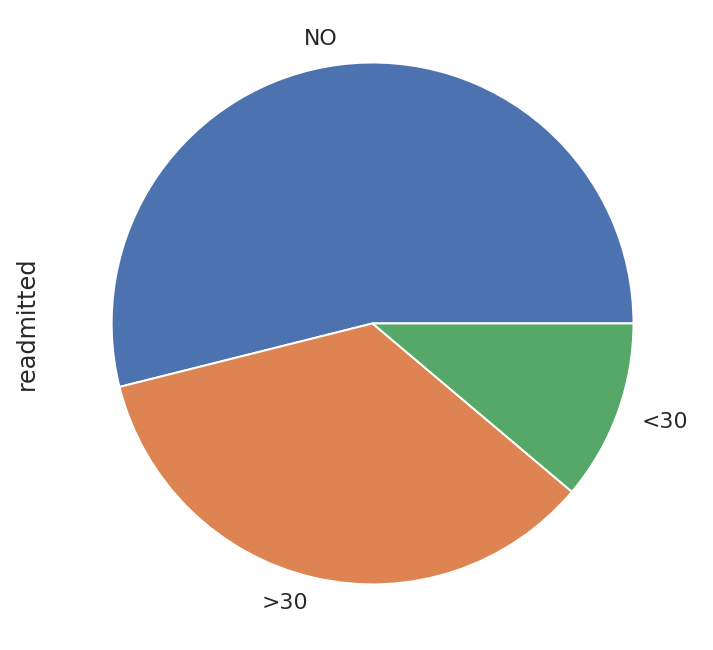
\includegraphics[width=\linewidth]{figures/classes_original.png}
        \caption{Original classes distribution}
        \label{fig:classes_original}
    \end{subfigure}%
    \begin{subfigure}{.5\textwidth}
        \centering
        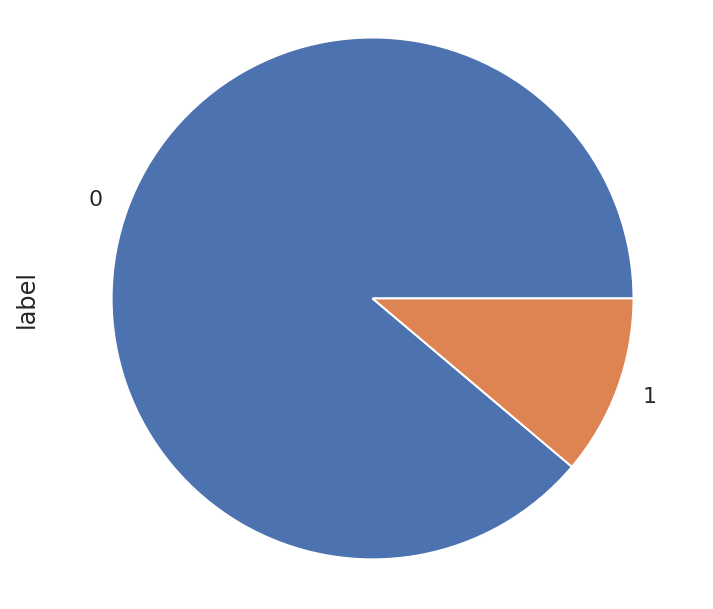
\includegraphics[width=\linewidth]{figures/classes_binary.png}
        \caption{Binary-converted classes distribution}
        \label{fig:classes_binary}
    \end{subfigure}
    \label{fig:classes_distribution}
    \caption{Distribution of predicted classes - original (whether and when was patient readmitted) and after converting to binary form (only whether was patient early readmitted or not).}
\end{figure}


\section{Data preprocessing}

During analysis of our dataset, some problems with data have been identified. To ensure reproducibility of preprocessing, data were preprocessed via \textit{pipeline}. Basic preprocessing steps based on data analysis results are included in pipeline:
\begin{enumerate}
    \item Drop redundant columns (or those with too low diversity, e.g. containing one major value). The columns with more than 45\% of missing values and columns where major value is present in more than 90\% cases are dropped. Also columns \textit{encounter id, patient number, payer code} that we observed as redundant are dropped.
    
    \item Merge too small classes in categorical attributes into one \textit{other} value, if there is less than 5\% values for class. 
    
    \item Fill missing values with most-frequent value for categorical attributes and median for numerical ones,
    
    \item Feature engineering (adding new features identified in data analysis). From attributes \textit{number emergency, number outpatient, number inpatient} and all attributes describing medicament we created new attributes: \textit{visits sum, number of medicaments changes} and \textit{total number of medicaments used}. Also, diagnoses codes had to be mapped into diagnoses categories (according to original paper~\cite{Strack2014}).
    
    \item Map ordinal features values into numbers (age categories we map into number values ordinary), 
    
    \item One-hot encoding (nominal attributes into numbers).
\end{enumerate}{}

We have checked numerical attributes carefully to see whether normalization and outliers removal should be performed. According to analysis, there are no such differences in measures so normalization is not needed. We have checked also outliers, but we have not found any extreme value that should be removed.


\section{Methods}

Our method to help to solve the task of early readmission prediction is based on basic machine learning workflow, using variety aspects of data mining methods.

With properly preprocessed data we did first experiments with three different types of machine learning  models like Random forest (RF), XGBoost and Multilayer perceptron (MLP).

\emph{Random forest} belongs to the group of tree based algorithms, which are one of the most popular in solving all kinds of data science problems. The building block of RF is Decision tree. Decision tree is tree structure, where each internal node denotes a test on an attribute, each branch represents an outcome of the test, and each leaf node represents a class label. 

A tree is learned by splitting training set into subsets by set of splitting rules based on classification features. This process repeats recursively on each derived subset while node contains only samples from one class or when splitting no longer adds value to the predictions. 

RF is  ensemble of many Decision trees. When RF predict class label, result is obtained by voting of all trees in the ensemble. We decided to use RF because  performs very well on the very large volume of data with high dimensionality. Next benefit is extraction of feature importance which can be helpful in models improving and feature selection.  

\emph{XGBoost} is also tree based algorithm containing set of Decision trees as above mentioned  Random forest. These models are very similar but main differences are in a way how trees are built and in combining results.

Random forest builds each tree independently while gradient boosting builds one tree at a time, where each new tree helps to correct errors made by previously trained tree. Random forests combine results at the end of the process while gradient boosting combines results along the way.

We decided to use XGBoost because it is an implementation of gradient boosted decision trees designed for speed and performance. Also, it is known as very powerful algorithm if it's parameters are carefully tuned. However, prone to over-fitting is one of the disadvantages of gradient boosted algorithms.

\emph{MLP} is a class of feedforward artificial neural network, containing at least three layers. One input and output layer, and multiple hidden layers consisting of multiple neurons. Each neuron in a layer is fully connected with all neurons from previous and next layer. Each neuron is weighted sum of outputs from neurons in previous layer with linear activation function.

Learning of MLP is based on changing connection weights in every data iteration, based on the amount of error in the output compared to the expected result. This is called loss, which is backpropagated and the weights of the model are updated by using gradient.

For reason we have identified neural networks in related works as one of the most powerful methods, we have chosen MLP as promising solution to problem of early readmission prediction.


\section{Evaluation}

\subsection{Methodology}
\label{sec:evaluation-methodology}
In the evaluation phase, we mainly focused on previously defined experiments with three types of machine learning algorithms. In the first step we split the data into train and test sets in ratio 80\%-20\%. Because the data we have chosen are highly imbalanced and only 11\% of the samples represent patient being early readmitted, we decided to experiment also with class balancing methods. 

As undersampling technique we used \emph{Random undersampling} that selects random samples from majority class to equal number of minority class samples. In case of oversampling we chose SMOTE technique that was mostly used in related works. SMOTE draws the line between the closest examples in feature space and generates new sample at a point along that line. With these data balancing techniques, only training set was balanced.

For complex comparison of how is each model performing, we used several evaluation metrics like F1-score, Precision, Recall and AUC ROC score. ROC curve consists of true positive rate (TPR or Recall, Sensitivity) and false positive rate (FPR or Fall-out) while positive class prediction probability threshold is varied. Figure \ref{fig:confusion-matrix} shows confusion matrix interpreting true positives, false positives, true negatives and false negatives.

\begin{figure}[h]
    \centering
    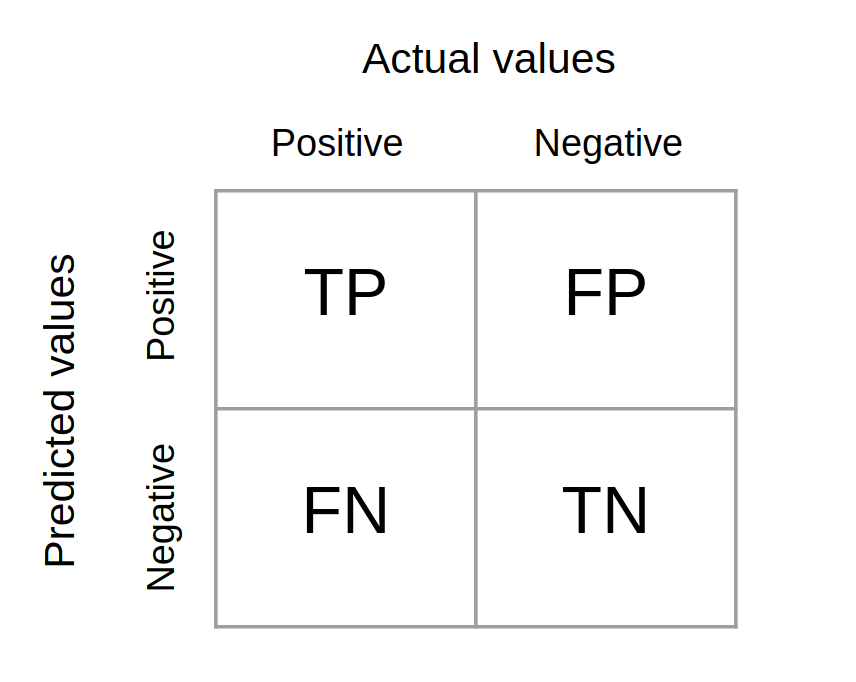
\includegraphics[width=0.5\linewidth]{figures/confusion_matrix.png}
    \caption{Confusion matrix.}
    \label{fig:confusion-matrix}
\end{figure}

\noindent Then, TPR and FPR are defined as follows:
$$TPR = \frac{TP}{TP + FN}$$

$$FPR = \frac{FP}{FP + TN}$$

All of mentioned metrics were calculated considering each class individually except AUC ROC score (that was calculated only considering positive class). We omitted Accuracy score because of highly imbalanced data. Precision, Recall and F1-score offer more realistic look at the model performance on each predicted group, however AUC ROC appears to be the most suitable metric considering mainly (but not only) positive class. Considering that, we have chosen AUC ROC as the main metric for final models comparison.

\subsection{Experiments results}
Table \ref{table:preliminary-results} shows the results of first experiments with Random forest, XGboost a MLP models. For each model, hyperparameters have been tuned only manually by intuition in this phase. Each of the models has been trained on three types of the data - original, undersampled and oversampled (with techniques mentioned in \ref{sec:evaluation-methodology}). We have achieved best results with Random forest on original data (with class weight parameter set to \textit{balanced}) and also the same model trained on undersampled data. Very similar results achieved XGBoost trained on original and undersampled data, alongside with MLP trained on all data variants. Results also showed that oversampling using SMOTE is not so much suitable for this data, even though majority of related works are using it. So, based on the results, we assume that the high scores achieved in the related works with SMOTE being used are due to oversampling also test set. We have tried also this setup and were able to achieve so high scores, but we consider this approach as incorrect.

\begin{table}
    \centering
    \caption{Results of first experiments - comparing Random forest, XGBoost and Multi-layer perceptron.\\\textbf{Note}: All metrics are calculated when considering early readmitted patients as positive class.}
    \begin{tabular}{ |l|c|c|c|c|c|c| } 
    \hline
    \textbf{Model} & \textbf{F1 (micro)} & \textbf{F1 (macro)} & \textbf{Precision} &  \textbf{Recall} &  \textbf{AUC ROC} \\
    \hline
    RF &   0.67    &   0.52    &   0.17    &   0.53   &   \textbf{0.65}\\
    RF undersampled &   0.60    &   0.49    &   0.16    &   0.63   &   \textbf{0.65}   \\
    RF oversampled &   0.42    &   0.38    &   0.13    &   0.75   &   0.60   \\
    \hline
    XGBoost &   0.52    &   0.45    &   0.15    &   0.69   &   0.64   \\
    XGBoost undersampled &   0.58    &   0.48    &   0.16    &   0.63   &   0.64   \\
    XGBoost oversampled &   0.42    &   0.38    &   0.12    &   0.69   &   0.57   \\
    \hline
    MLP &   0.89    &   0.49    &   0.41    &   0.02   &   0.64   \\
    MLP undersampled &   0.63    &   0.50    &   0.16    &   0.56   &   0.64   \\
    MLP oversampled &   0.89    &   0.49    &   0.35    &   0.02   &   0.64   \\
    \hline
    \end{tabular}
    \label{table:preliminary-results}
\end{table}

In next phase of experiments, we have tried also three ensemble techniques - \textit{Bagging}, \textit{Voting} and \textit{Stacking}. We expected that any kind of several models combination can give as better and more stable predictions. In all of these ensemble-based experiments, algorithms were trained on undersampled data only, as this setup seemed to be the best (according to previous results).

As a base classifier for Bagging method, we selected Random forest with manually chosen hyper-parameters setup from previous experiments. For other both methods, Voting and Stacking, we used all previous tested models - Random Forest, XGBoost and MLP. In Stacking method, simple \textit{Logistic Regression} was used to combine the classifiers. Table \ref{table:ensemble-results} shows results for all ensemble methods. As can be seen in the table, none of the ensemble methods significantly improved the prediction performance. 
\begin{table}
    \centering
    \caption{Results of experiments with ensemble methods.\\\textbf{Note}: All metrics are calculated when considering early readmitted patients as positive class.}
    \begin{tabular}{ |l|c|c|c|c|c|c| } 
    \hline
    \textbf{Model} & \textbf{F1 (micro)} & \textbf{F1 (macro)} & \textbf{Precision} &  \textbf{Recall} &  \textbf{AUC ROC} \\
    \hline
    Bagging &   0.60    &   0.49    &   0.16    &   0.64   &   0.65\\
    Voting &   0.62    &   0.50    &   0.16    &   0.60   &   0.65\\
    Stacking &   0.62    &   0.50    &   0.17    &   0.61   &   0.65\\
    \hline
    \end{tabular}
    \label{table:ensemble-results}
\end{table}

For final evaluation phase, Random forest in combination with data balancing using random undersampling has been chosen because of achieved results, the speed and the simplicity (in comparison to other algorithms). Even though ensemble methods achieved almost the same results, Random forest is preferred because of it's simplicity. In the final evaluation phase, firstly feature selection was performed using \textit{Recursive Feature Elimination with Cross-Validation}. The process of finding optimal number of features is shown in figure \ref{fig:feature-selection}. As can be seen at the plot, majority of features has been chosen (49 out of 54 features).

\begin{figure}[h]
    \centering
    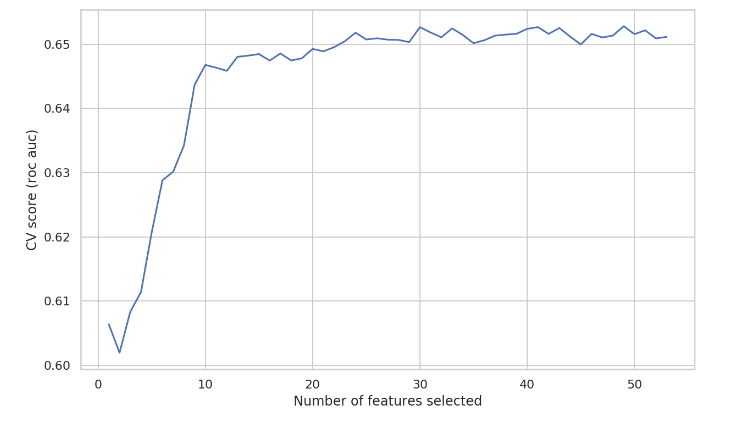
\includegraphics[width=0.9\linewidth]{figures/feature_selection.png}
    \caption{Finding optimal number of features with RFECV.}
    \label{fig:feature-selection}
\end{figure}

After feature selection, hyperparameters of Random forest were optimized with \textit{Random search}, while using only best-selected features from feature selection. Final model with optimized hyperparameters achieved ROC AUC equal to 0.65, that was achieved also without parameters optimization. The learning curve of final model with optimized hyperparameters and using only selected features is shown in figure \ref{fig:learning-curve}. From the learning curve we can conclude, that adding more data and features may help to achieve even better results. The confusion matrix and ROC curve of final model is shown in figure \ref{fig:final-model-results}.

\begin{figure}[h]
    \centering
    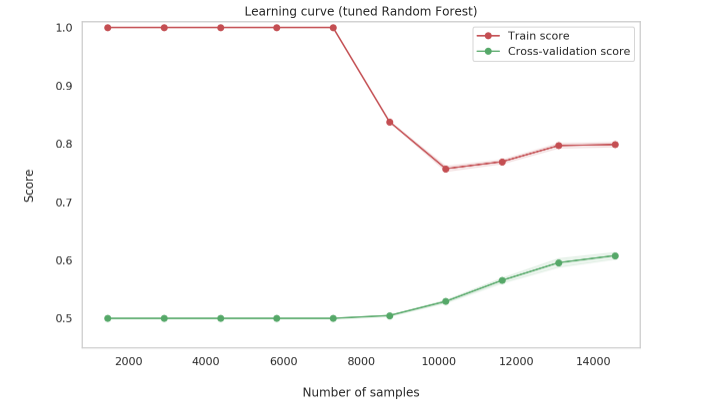
\includegraphics[width=0.9\linewidth]{figures/learning_curve.png}
    \caption{Learning curve of final model - Random forest with optimized hyperparameters. Model was trained on balanced data using random undersampling with only features selected by RFECV.}
    \label{fig:learning-curve}
\end{figure}

\begin{figure}[h!]
    \centering
    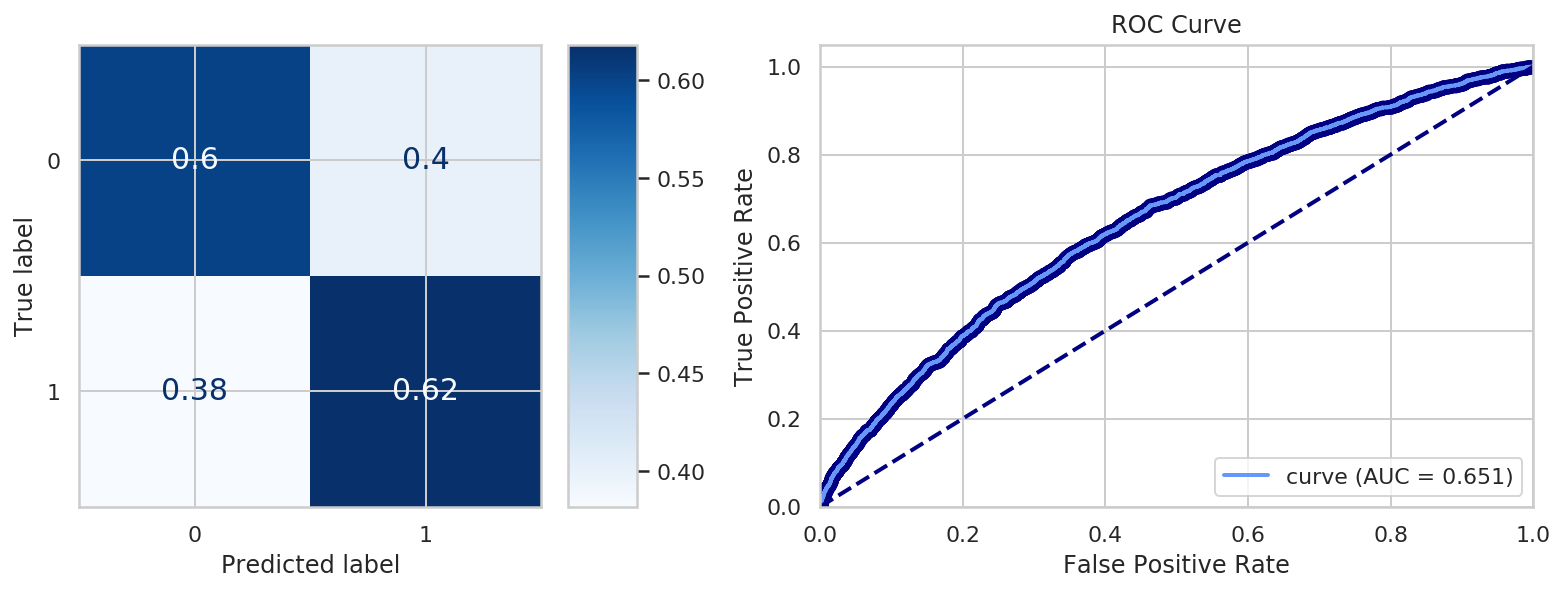
\includegraphics[width=\linewidth]{figures/final_model.png}
    \caption{Confusion matrix and ROC curve of final model.}
    \label{fig:final-model-results}
\end{figure}

Any of the previous efforts to boost up performance of baseline model were not successful. The problem may stem from the nature of the data. Some complementary experiments focused on dividing data to subsets were performed - either using natural subsets existing in the data or using clustering.

As a first approach, data were divided according to age into four age intervals. Then, four individual models (again RF) were trained on samples from corresponding interval. Then, the new samples from test set are predicted with appropriate model according to their age. No significant improvements have been achieved, but at least new information about the nature of the data were observed. Results from individual age intervals showed trend, that performance of model is decreasing with increasing age. Simply, older patients are harder to be predicted. This observation was also mentioned in several related works. For patients under age of 50 and also at age from 50 to 70, models achieved significantly better results in comparison to model trained on all samples (not divided by age). However, models trained on older patients decreased the overall performance.

In the second complementary experiment, data were clustered using KMeans clustering algorithm. Within each individual cluster, one model was trained. The unseen sample from test set is firstly classified to one of the clusters, then the label is predicted with appropriate model. Again, no improvements were observed.


\section{Conclusion}

In this work, we used data-mining approach to predict diabetic patients early readmission. To train the machine learning model for this problem, we have chosen popular dataset of diabetes patients clinical encounters across 130 hospitals in United States. Based on the comprehensive data analysis, we have preprocessed the data and create new features. In model selection phase, experiments with Random forest, XGBoost and Multi-layer perceptron were conducted. Each algorithm was trained on three data setups - original imbalanced data, the data balanced with random undersampling and oversampling using SMOTE method. Random forest turned out to be the best performing, so was chosen for final optimization and evaluation. Feature selection using Recursive Feature Elimination with Cross-Validation and hyperparameters optimization using Random search were performed to obtain final model. The final model was trained on undersampled balanced data and achieved ROC AUC score equal to 0.65. Multiple complementary experiments were conducted to boost up the score - ensemble models or dividing data into subsets by either age or clustering. However, no significant improvements were observed. We also analyzed several of related papers where data balancing techniques (SMOTE mostly) boosted the performance of model up to more than 90 percent ROC AUC. We found out that all of those works have applied SMOTE on whole dataset before train-test splitting. This approach leads model to learn to classify SMOTE algorithm instead of real classification problem, that we consider incorrect. Despite several methods that were tried, we were not able to obtain better model. Thus, for the future work we mainly propose to explore more datasets in this area to build better models.


% ---- Bibliography ----
%
% BibTeX users should specify bibliography style 'splncs04'.
% References will then be sorted and formatted in the correct style.
\bibliographystyle{splncs04}
\bibliography{references}

\end{document}
